\chapter{Diseño e implementación del sistema IoT} % Main chapter title

\label{Chapter3} % Change X to a consecutive number; for referencing this chapter elsewhere, use \ref{ChapterX}

En este capítulo se detallan las consideraciones de diseño que se tuvieron en cuenta para realizar el sistema IoT y se describe el desarrollo y servicios implementados para este trabajo.



%----------------------------------------------------------------------------------------
%	SECTION 1
%----------------------------------------------------------------------------------------


\section{Diseño general del sistema}

Como se observa en la figura \ref{fig:arquitectura}, el sistema está compuesto por una arquitectura que integra cuatro componentes necesarios para su funcionamiento, los dispositivos (sensores y actuadores), el servidor local, los elementos de red y el servicio en la nube.

El diseño del sistema se basó en una arquitectura distribuida donde se despliegan distintas tecnologías de \emph{hardware} y \emph{software} con el objetivo de ofrecer acceso desde dentro o fuera de la red doméstica del edificio. La interfaz de comunicación con el servidor interno y externo se hizo mediante el protocolo MQTT por ser ligero y de bajo consumo de ancho de banda para la red \emph{wireless} utilizada. 

La etapa de diseño se inició con la modelización de los componentes más importantes del sistema IoT, que son los módulos sensores y actuadores. En un segundo paso se desarrolló el software de monitoreo web, según patrones de diseño y características para garantizar la seguridad de la aplicación web. 

Para el diseño e implementación de \emph{firmware} se utilizó Arduino teniendo en cuenta patrones y conceptos de la programación funcional. La comunicación MQTT se realizó mediante la biblioteca PubSubClient versión 2.7.0 \citep{WEBSITE:46} y la visualización gráfica de las pantallas OLED y GLCD, con las bibliotecas Adafruit GFX versión 1.7.2 \citep{WEBSITE:47} y U8g2\_for\_Adafruit\_GFX versión 2.28.10 \citep{WEBSITE:48} respectivamente.


Como se eligió el protocolo MQTT para la comunicación entre módulos y el conjunto de servicios, se definieron tres tipos de tópicos para poder comunicarse entre sí. Estos tópicos son:

\begin{itemize}

\item Tópico de envió de valores: permite que un módulo envíe un dato JSON con valores de su sensor hacia el servidor local.  La figura \ref{fig:comunica1} muestra la lógica de su aplicación en la comunicación.
%Solamente utilizado mediante comunicación unidireccional.

\item Tópico de comunicación de estados: es utilizado por todos los módulos y permite el envió de un dato JSON con valores de su estado actual desde el sensor o actuador hacia el servidor local. La figura \ref{fig:comunica1} muestra la lógica de su aplicación en la comunicación.
%Solamente utilizado mediante comunicación unidireccional.

%%%%%%%%%%%%%%%%%%%%%%%%%%% imagen horizontal%%%%%%%%%%%%%%%%%%%%%%%%%%%%%%%%%%%%%%%%%%%%
\begin{landscape} % esto es para rotar la pagina e imagen
\begin{figure}[htpb]
\centering 
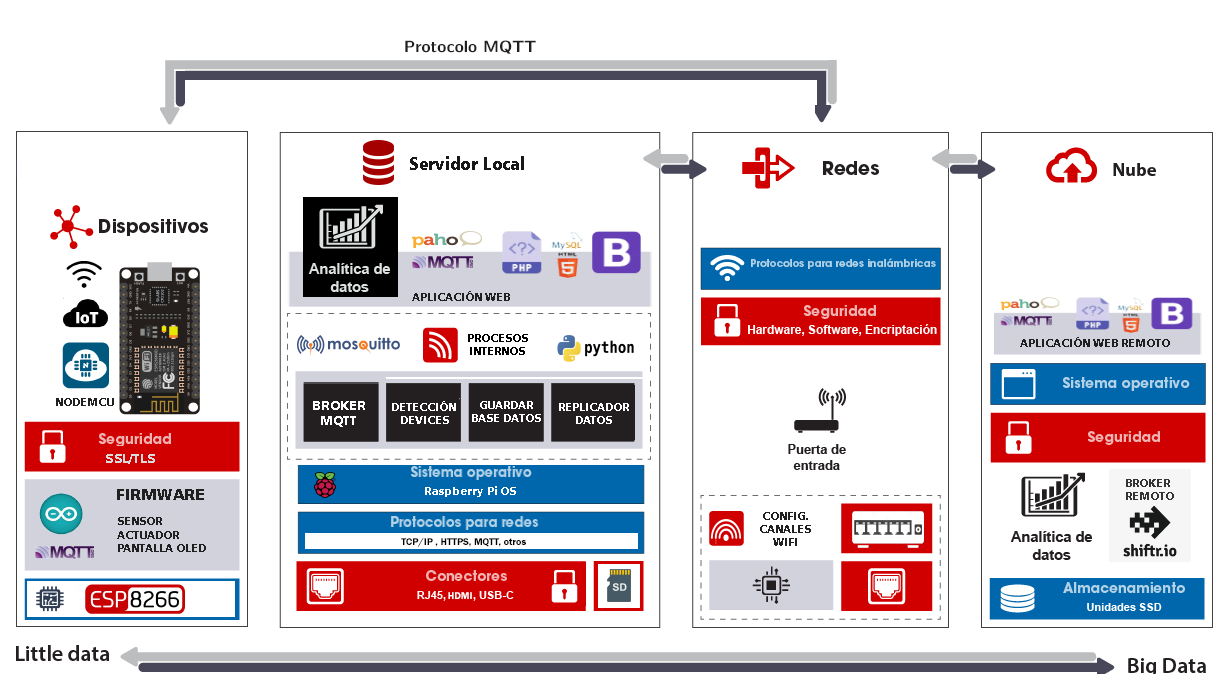
\includegraphics[width=1.65\textwidth]{./Figures/arquitectura-listo.png}
\caption{Arquitectura del sistema IoT.}
\label{fig:arquitectura}
\end{figure}
\end{landscape} % esto es para rotar
%%%%%%%%%%%%%%%%%%%%%%%%%%%%%%%%%%%%%%%%%%%%%%%%%%%%%%%%%%%%%%%%%%%%%%%%%%

%\vspace{1cm}
\begin{figure}[htpb]
\centering 
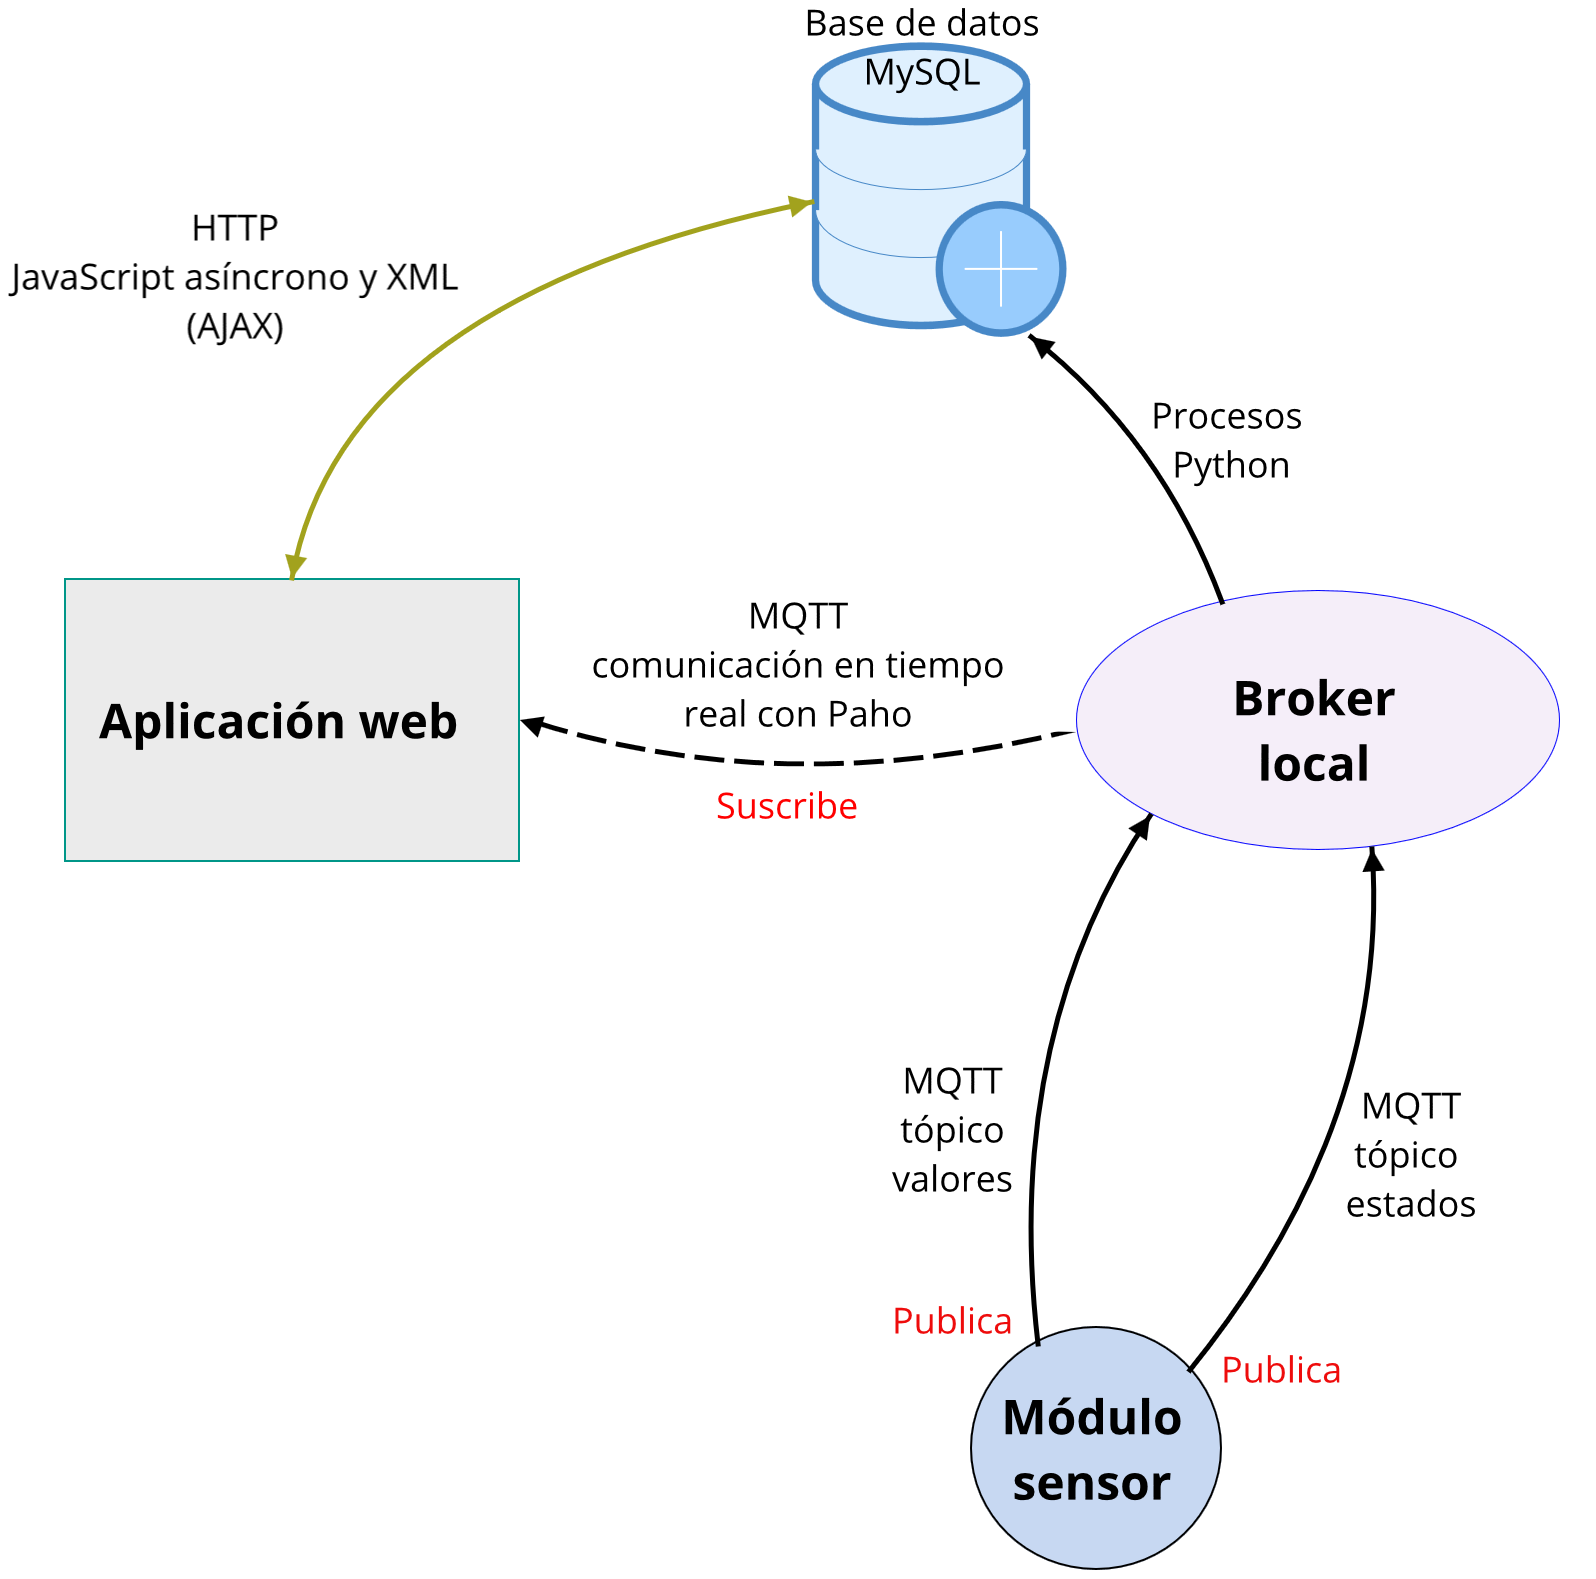
\includegraphics[width=0.6\textwidth]{./Figures/sensores.png}
\caption{Lógica de comunicación MQTT del módulo sensor.}
\label{fig:comunica1}
\end{figure}


\item Tópico de sincronización: permite que un módulo envíe un dato JSON para actualizar información en todos los módulos suscriptos al tópico. Es utilizado en la comunicación entre el \emph{software} de monitoreo, los actuadores y el broker del servidor local. La figura \ref{fig:comunica2} muestra la lógica de su aplicación en la comunicación.
\end{itemize}


\begin{figure}[htpb]
\centering 
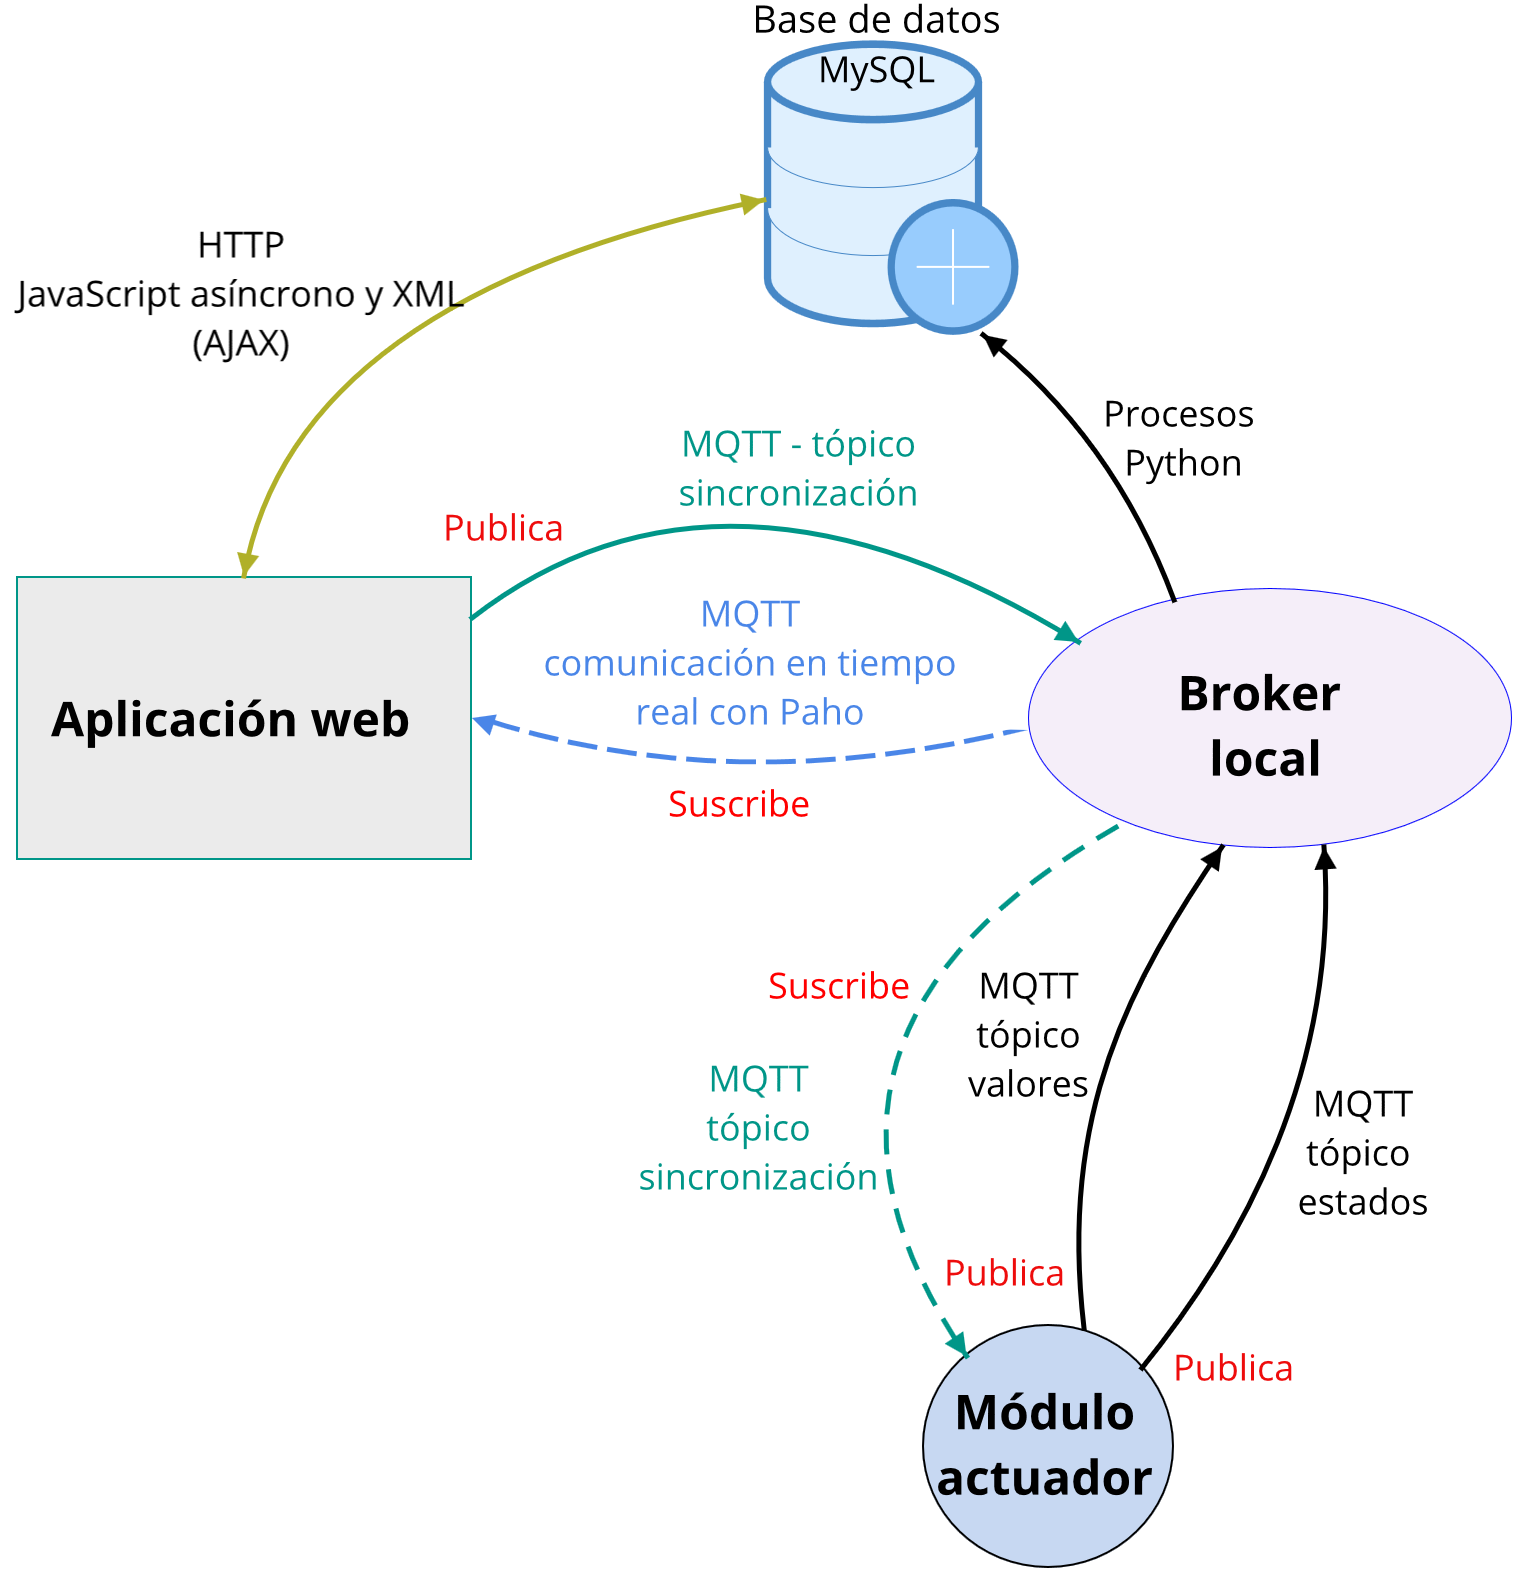
\includegraphics[width=0.6\textwidth]{./Figures/actuadores.png}
\caption{Lógica de comunicación MQTT del módulo actuador.}
\label{fig:comunica2}
\end{figure}




El software de monitoreo de tipo web local y remoto fue diseñado y desarrollado a medida para garantizar dominio total de la plataforma usada. Utiliza el \emph{framework bootstrap} para lograr interfaces gráficas de usuario que cumplan con los principios de experiencia de usuario (UX) y compatibilidad de dispositivos. Para la recepción de mensajes se usó web sockets mediante \emph{JavaScript} teniendo configurado los tres tópicos de comunicación antes mencionados para el intercambio de mensajes con los módulos.

La figura \ref{fig:diagrama_general} muestra el diagrama general del funcionamiento del sistema desde la perspectiva conceptual. El desarrollo, consideraciones de construcción y fabricación para cada módulo del sistema se describen en detalle en las siguientes secciones de este capítulo.


\begin{figure}[htbp]
	\centering
	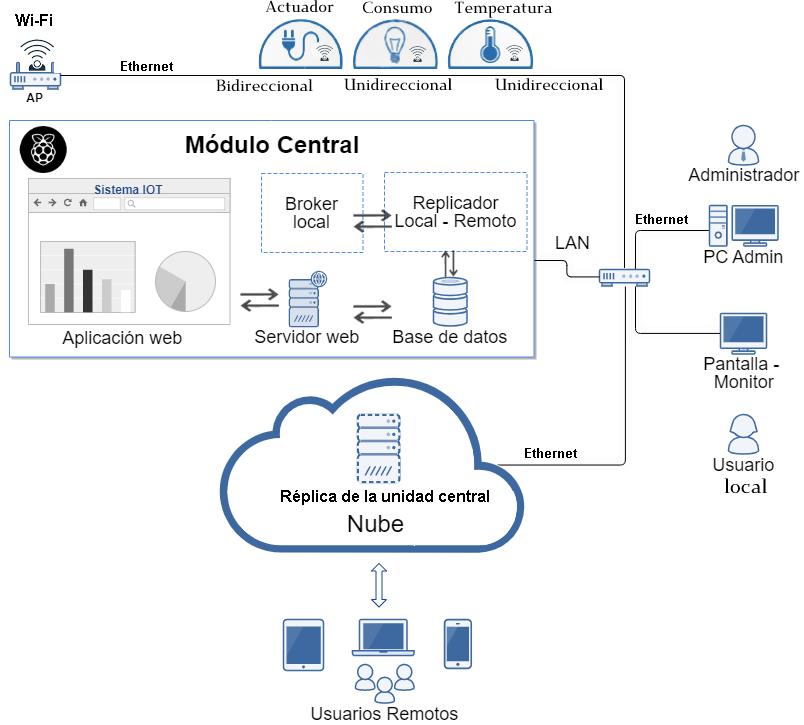
\includegraphics[width=0.9\textwidth]{./Figures/diagrama0.png}
	\caption{Diagrama general del funcionamiento del sistema.}

	\label{fig:diagrama_general}
\end{figure}

%\vspace{0.5cm}


%\section{Medidas de ciberseguridad}

%Los requerimientos de ciberseguridad dentro del desarrollo ocupan un lugar muy importante en cada una de las etapas ejecutadas en el proceso de implementación de un sistema IoT, porque permite garantizar un grado mínimo de seguridad y confiabilidad funcional del producto. 

%Los requerimientos considerados durante el proceso, son los siguientes:





%\subsection{Requerimientos para los módulos IoT}
%Se buscó cumplir con los requerimientos que se plantean a continuación:

%\begin{itemize}
%\item Uso de programación basada en código modular para el desarrollo del \emph{firmware}.
%\item Uso de la biblioteca en su versión más actual para la comunicación MQTT.
%\item Los objetos de datos a transmitir serán del formato JSON.
%\item La comunicación el protocolo MQTT debe contener TLS.
%\end{itemize}





%\section{Construcción y programación de módulos}

%En esta sección se describen el proceso y consideraciones técnicas para la construcción de cada uno de los módulos del sistema IoT propuesto.
%%%%%%%%%%%%%%%%%
\section{Módulo principal}

El módulo principal representa el elemento central dentro de la solución IoT planteada y para  su construcción e instalación se utilizaron recursos que hicieron posible una versión de fácil uso para el usuario. Las consideraciones generales de seguridad para el módulo principal fueron:

\begin{itemize}
\item Sistema operativo GNU/Linux oficial Raspberry Pi OS \citep{WEBSITE:44}\citep{WEBSITE:45}.
\item Acceso al sistema operativo mediante usuario y contraseña.
\item Accesos remotos por SSH (\emph{Secure Shell}) y FTP (\emph{File Transfer Protocol})  desactivados.
\item Cifrado de las unidades de almacenamiento del sistema operativo.
\end{itemize}

La figura \ref{fig:argon} muestra la integración y ensamblado del módulo principal.

%%%%%%%%%%%%%%%%%%%%%%%%%%% imagen horizontal%%%%%%%%%%%%%%%%%%%%%%%%%%%%%%%%%%%%%%%%%%%%
%\begin{landscape} % esto es para rotar la pagina e imagen
\begin{figure}[htpb]
\centering 
%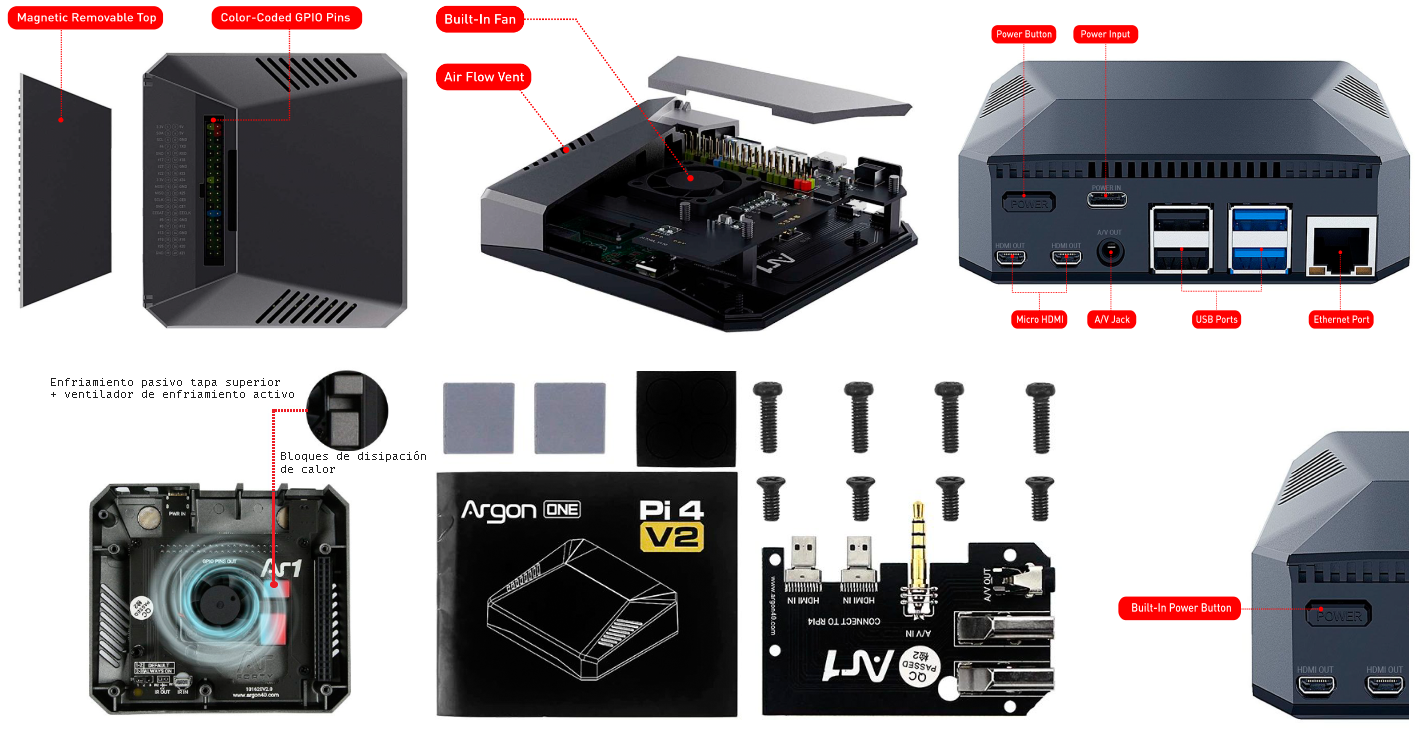
\includegraphics[width=1.7\textwidth]{./Figures/argon.png}
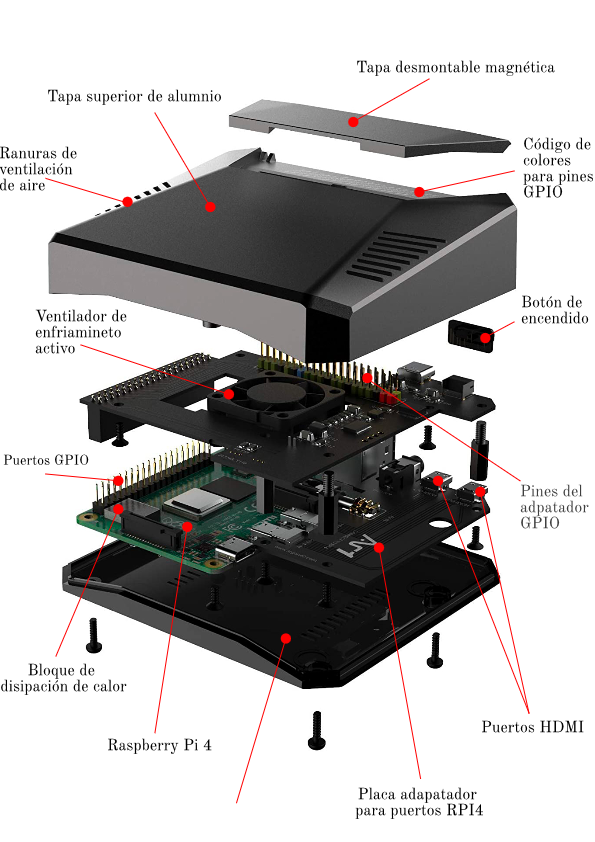
\includegraphics[width=0.92\textwidth]{./Figures/armadoactuador.png}
\caption{Ensamblado y partes del módulo principal. }
\label{fig:argon}
\end{figure}
%\end{landscape} % esto es para rotar
%%%%%%%%%%%%%%%%%%%%%%%%%%%%%%%%%%%%%%%%%%%%%%%%%%%%%%%%%%%%%%%%%%%%%%%%%%%





%Las consideraciones de seguridad para la configuración del broker fueron:

%\begin{itemize}
%\item Configuración de usuario y contraseña para controlar el acceso a los canales de comunicación del broker local y remoto.
%\item Uso de canales separados, para el envió, sincronización y respuesta entre elementos del sistema IoT.
%\item Cada mensaje debe ir con destino a un tópico en específico, evitar envió de datos a la instancia general \#.
%\item Configurar permisos para la edición o ejecución a los archivos de configuración del broker.
%\end{itemize}


\section{Módulo replicador a la nube}

El módulo replicador a la nube está dentro del módulo principal y para su desarrollo se diseñó una estructura interna compuesta por subprocesos que, al trabajar en conjunto, forman el sistema completo de replicación.

La replicación solo se da mientras exista conexión a Internet. El desarrollo de cada subproceso se programó en Python por tratarse de un lenguaje multiplataforma, robusto y orientado a objetos. La figura \ref{fig:logicareplicador} ilustra la lógica de trabajo del replicador.


%\begin{figure}[htpb]
%\centering 
%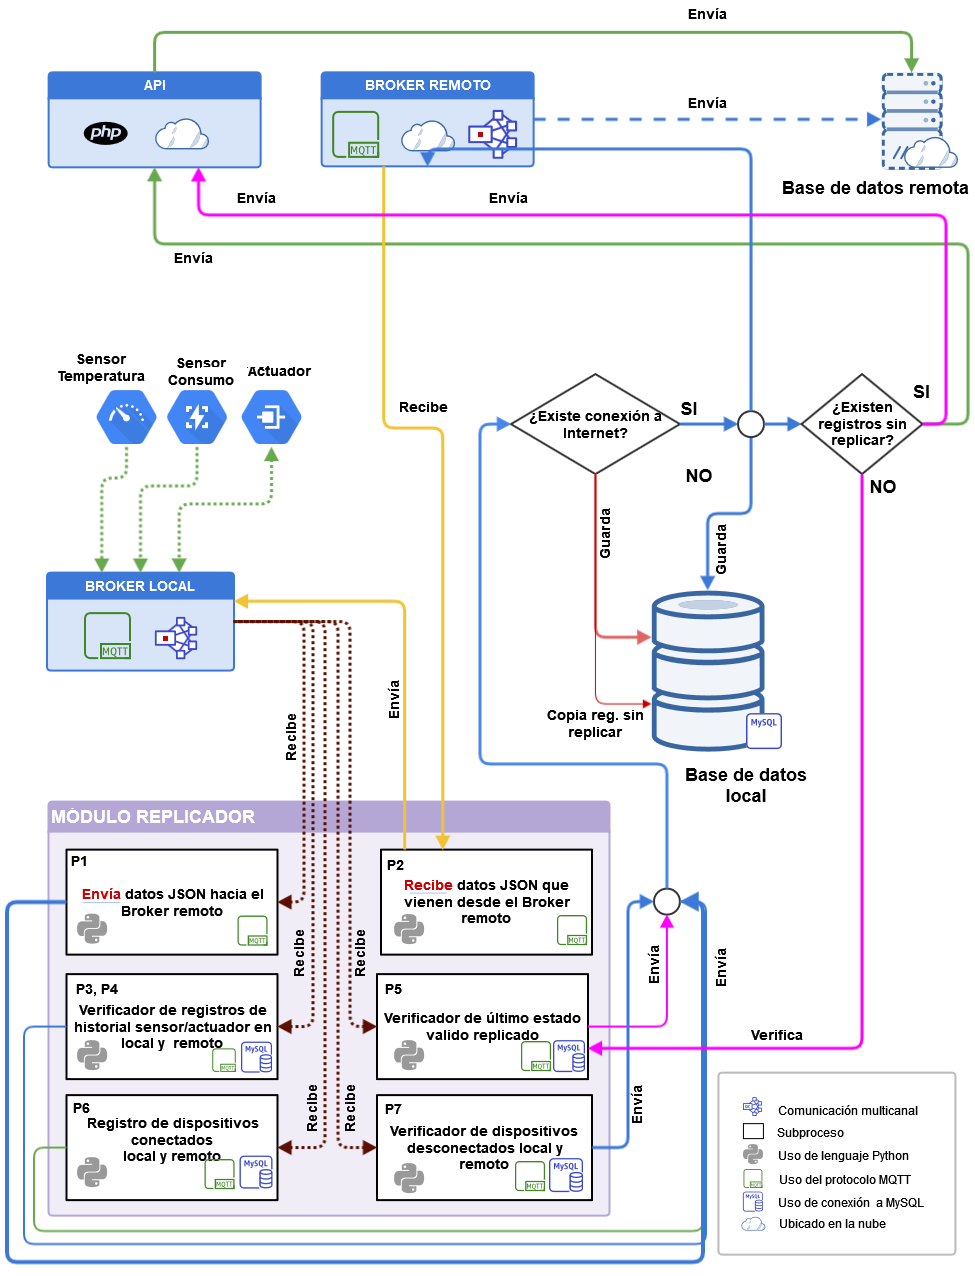
\includegraphics[width=1.15\textwidth]{./Figures/replicador.png}
%\caption{Flujo funcional del módulo replicador.}
%\label{fig:flujoreplicador}
%\end{figure}



Las descripciones de cada subproceso interno que contiene el módulo replicador se detallan a continuación usando el nombre del proceso con el cual fue creado: 

\begin{itemize}
\item \keyword{mqtt\_envia\_nube\_poo (P1)}: es el responsable de reenviar al broker remoto todos los mensajes que llegan al broker local. Se usa el formato JSON.

\item \keyword{mqtt\_recibe\_nube\_poo (P2)}: es el responsable de recibir los datos JSON que fueron generados en la aplicación web remota y que llegan desde el broker remoto para luego enviarlos al broker local.

\item \keyword{actuador\_registros\_bd (P3)}: es el responsable de verificar los registros en la base de datos. La verificación se realiza en intervalos de tiempo de una hora. Consulta todos los registros de lecturas de actuadores dentro de una hora específica en las tablas auxiliares de actuadores y consumos, luego obtiene la media de los consumos y hace un solo registro en la tabla de historial de consumo. Finalmente realiza el borrado de los registros temporales utilizados.

\item \keyword{sensor\_registros\_bd (P4)}: es el responsable de verificar los registros en la base de datos. La verificación se realiza en intervalos de tiempo de una hora, consulta todos los registros de lecturas de sensores dentro de una hora específica en las tablas auxiliares de sensores, luego obtiene la media de los registros y hace un solo registro en la tabla de historial de sensores. Finalmente realiza el borrado de los registros temporales utilizados.

\item \keyword{sensor\_historial\_replicas\_bd (P5)}: es el responsable de verificar de forma constante la conexión a Internet y si existen datos por replicar. En caso de disponer de una conexión a Internet y a partir de registros marcados como no replicado procede a enviar los últimos registros hacia la nube. Finalmente actualiza en el campo de la tabla de registros\_no\_enviados, y así se mantiene la consistencia necesaria entre el sistema local y remoto.

\item \keyword{mqtt\_gestionBD\_poo (P6)}: es el responsable de recibir todos los mensajes que llegan al broker y verificar la pertenencia del JSON capturado (sensor o actuador). Posteriormente, comprueba si existe conexión a Internet. En el caso que no esté disponible la conexión solo se hace el registro en la tabla local y se lo marca como no replicado, para que pueda ser enviado a la nube cuando vuelva a existir la conexión a Internet. Este subproceso también permite actualizar el estado de un sensor o actuador en la base de datos con el estado de ``CONECTADO'' mientras esté activo en la red.

%\vspace{0.05cm}
%%%%%%%%%%%%%%%%%%%%%%%%%%% imagen horizontal%%%%%%%%%%%%%%%%%%%%%%%%%%%%%%%%%%%%%%%%%%%%
\begin{landscape} % esto es para rotar la pagina e imagen
\begin{figure}[htbp]
	\centering
	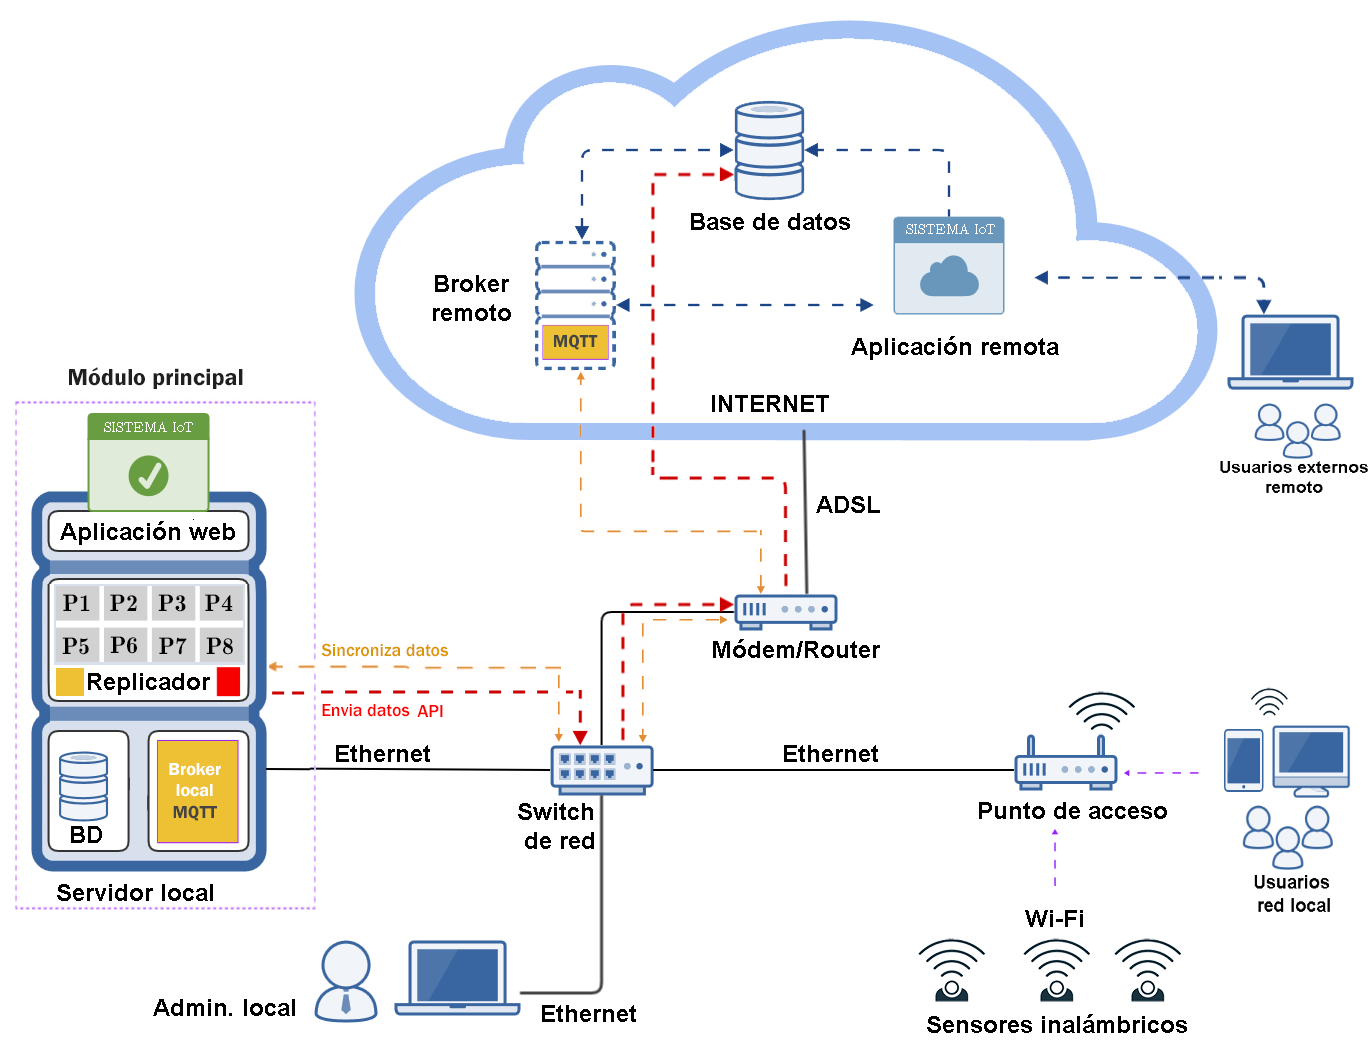
\includegraphics[width=1.2\textwidth]{./Figures/diagrama2.png}
	\caption{Diagrama funcional del replicador. }

	\label{fig:logicareplicador}
\end{figure}
\end{landscape} % esto es para rotar
%%%%%%%%%%%%%%%%%%%%%%%%%%%%%%%%%%%%%%%%%%%%%%%%%%%%%%%%%%%%%%%%%%%%%%%%%%%

\item \keyword{mqtt\_gestionDispositivosConectados (P7)}: es el responsable de recibir todos los mensajes que llegan al broker, verificar la pertenencia del JSON capturado (sensor o actuador) para registrar temporalmente el tiempo de llegada del mensaje del dispositivo. 

Este subproceso usa hilos en Python para estar constantemente registrando los tiempos de llegada de mensajes de cada sensor o actuador, y si los intervalos de tiempo de llegada de mensajes para un dispositivo activo son mayores a un minuto, el subpoceso actualiza el estado del dispositivo con el estado de ``DESCONECTADO'' en la base de datos.

\item \keyword{sensorEstadoRed (P8)}: es el responsable de verificar el estado del servicio de Internet en la red WLAN. Este subproceso usa hilos en Python para registrar periódicamente en la base de datos el estado actual de la red interna.

\end{itemize}

\section{Módulo de medición de temperatura}

Este módulo permite recoger lecturas de temperatura y humedad en ambientes de un hogar, oficina o edificio. Los valores son enviados y procesados en el sistema IoT de control y monitoreo que se encuentra en el servidor web del módulo principal. Las lecturas de temperatura son utilizadas para conocer la curva de cambios de temperatura según el horario registrado, así como su relación directa con el consumo eléctrico por el uso de ventiladores y equipos de aire acondicionado. Para su construcción se usó la placa NodeMCU8266 V3, por su capacidad de conexión inalámbrica. 

Este módulo integra una pantalla SSD1306 OLED para visualizar el valor de la temperatura en tiempo real. Para el encapsulado y construcción se utilizó un tablero adosable de montaje de interruptores térmicos y diferenciales tipo RIEL-DIN, de material de poliestireno y cubierta trasparente de policarbonato con apertura vertical \citep{WEBSITE:17}, como se aprecia en la figura \ref{fig:casetemp}.


\begin{figure}[htpb]
\centering 
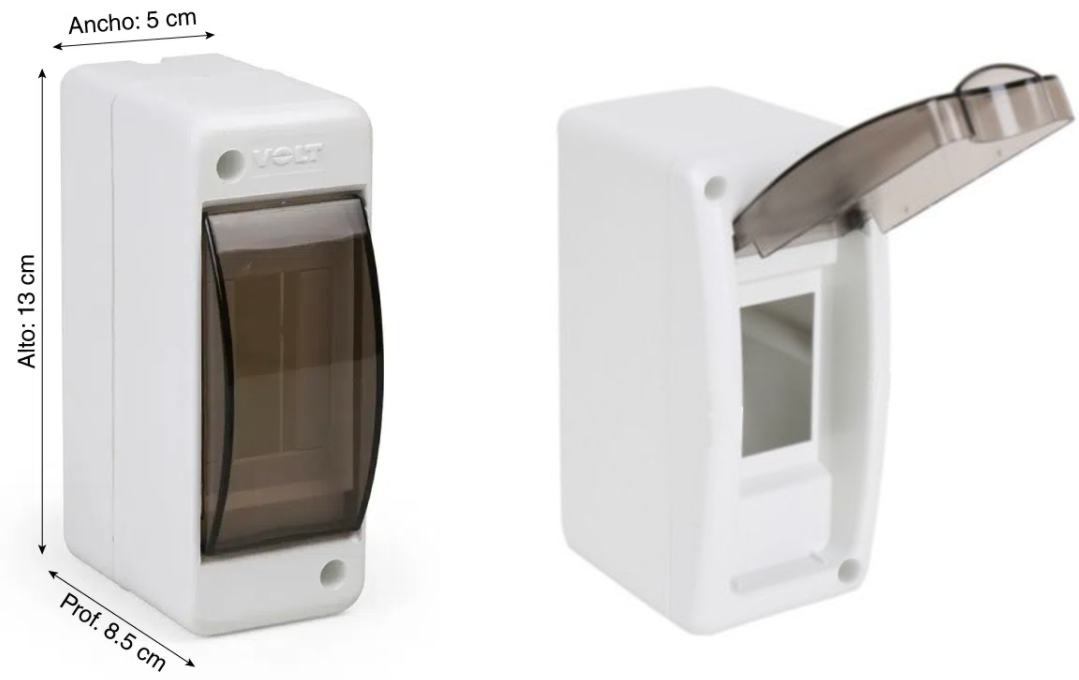
\includegraphics[width=0.7\textwidth]{./Figures/casetemp.png}
\caption{Case del módulo de temperatura \protect\footnotemark.}
\label{fig:casetemp}
\end{figure}

\footnotetext{Imagen tomada de \url{https://www.promart.pe/tablero-2-polos-adosable-c-puerta/p}}

El diseño de integración de componentes electrónicos se realizó en una Placa PCB perforada siguiendo el esquemático de la figura \ref{fig:citemp}.

\begin{figure}[htpb]
\centering 
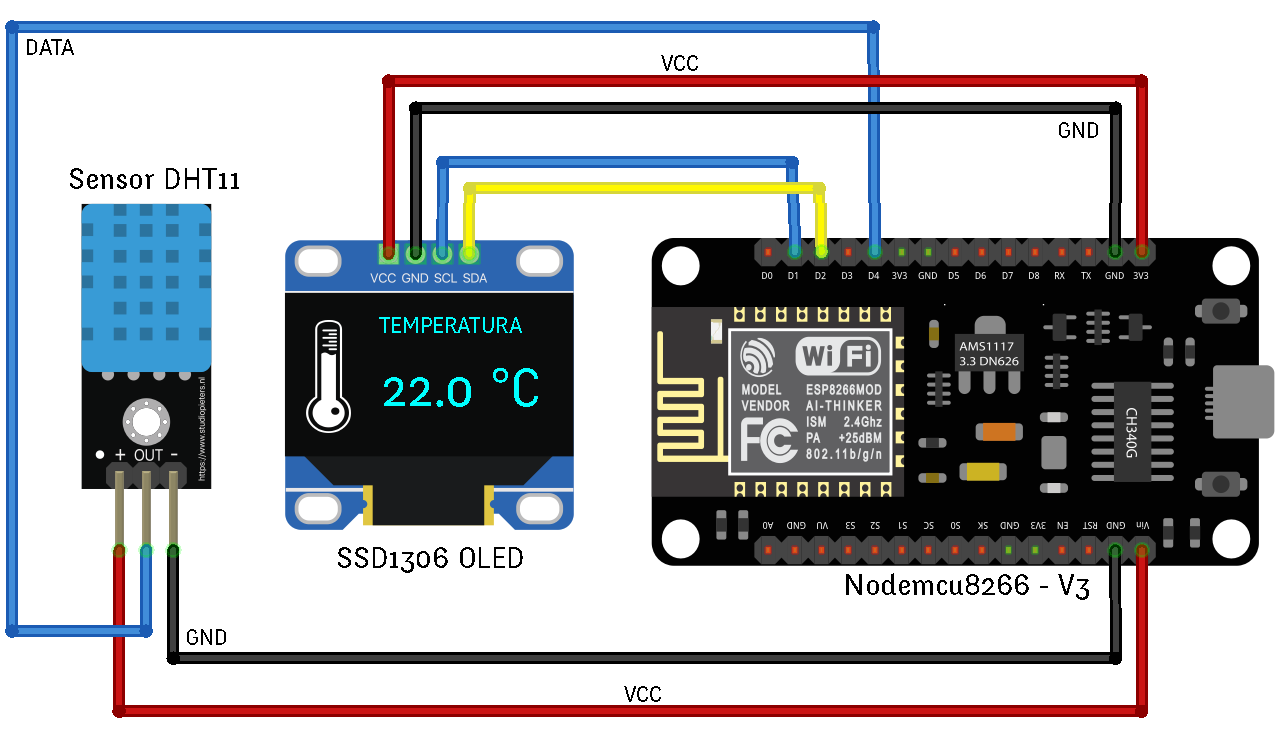
\includegraphics[width=0.85\textwidth]{./Figures/ci-temp.png}
\caption{Esquemático electrónico del módulo de temperatura. }
\label{fig:citemp}
\end{figure}

\vspace{0.5cm}
El proceso de integración se puede ver en la figura \ref{fig:entemp}.

\begin{figure}[htpb]
\centering 
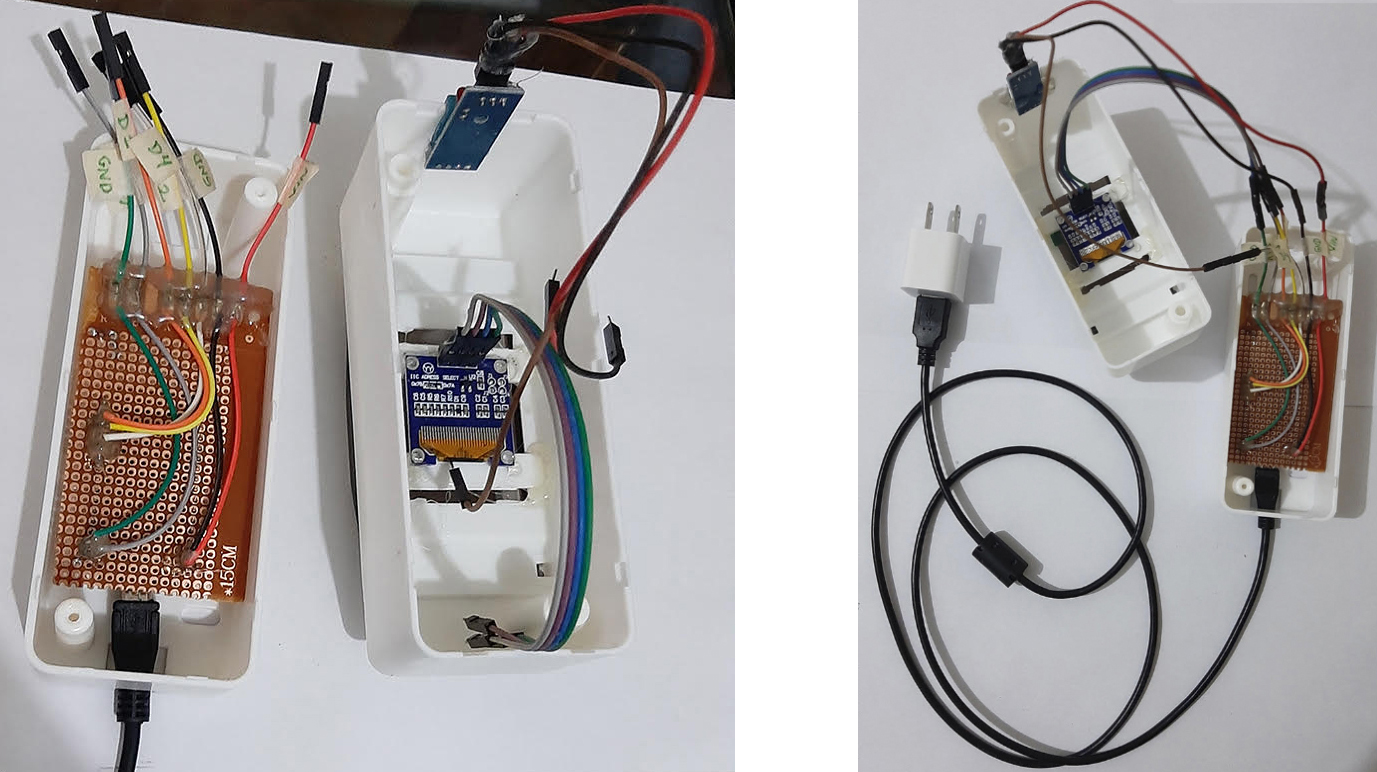
\includegraphics[width=0.95\textwidth]{./Figures/temperatura.jpg}
\caption{Ensamblado del módulo de temperatura. }
\label{fig:entemp}
\end{figure}

\section{Módulo actuador}

Este módulo permite activar o desactivar el paso de la corriente eléctrica dentro de un tomacorriente. La acción de cambio de estado (activado o desactivado) se realiza desde un switch en la interfaz de la aplicación web de monitoreo y control. El software envía un mensaje JSON por medio del canal de sincronización con el código y número de modelo del relé a activar o desactivar.

Para la construcción del módulo se utilizó una caja de tomacorriente  resistente a impactos, de gran durabilidad, autoextinguible e ideal para conductos de cables \citep{WEBSITE:18}. Para fijar el tomacorriente se usó una placa modular de soporte. En la figura \ref{fig:caseactuador} se ilustran los componentes mencionados.

%El corte o paso de energía eléctrica se realiza desde el software de monitoreo mediante el componente \emph{Toggle Switch} para activar o desactivar el relé. 

Para la activación del relé de 5 V mediante la salida de la placa NodeMCU8266 fue necesario usar un convertidor de tensión DC-DC Step-Up 2 A MT3608, porque las salidas de la placa NodeMCU8266 son de 3,3 V y la activación del relé requiere 5 V para funcionar. La figura \ref{fig:esquemaactuador} ilustra el relé de 30 A y el convertidor de tensión utilizado para la solución a este problema.


%El DC-DC Step-Up tiene como función entregar una tensión de salida constante superior a la tensión de entrada, soporta como tensión de entrada entre 2 V a 24 V y tensión de salida entre 2 V a 28 V. La tensión de salida se puede regular mediante un potenciómetro multivuelta \citep{WEBSITE:19}. 


\begin{figure}[htpb]
\centering 
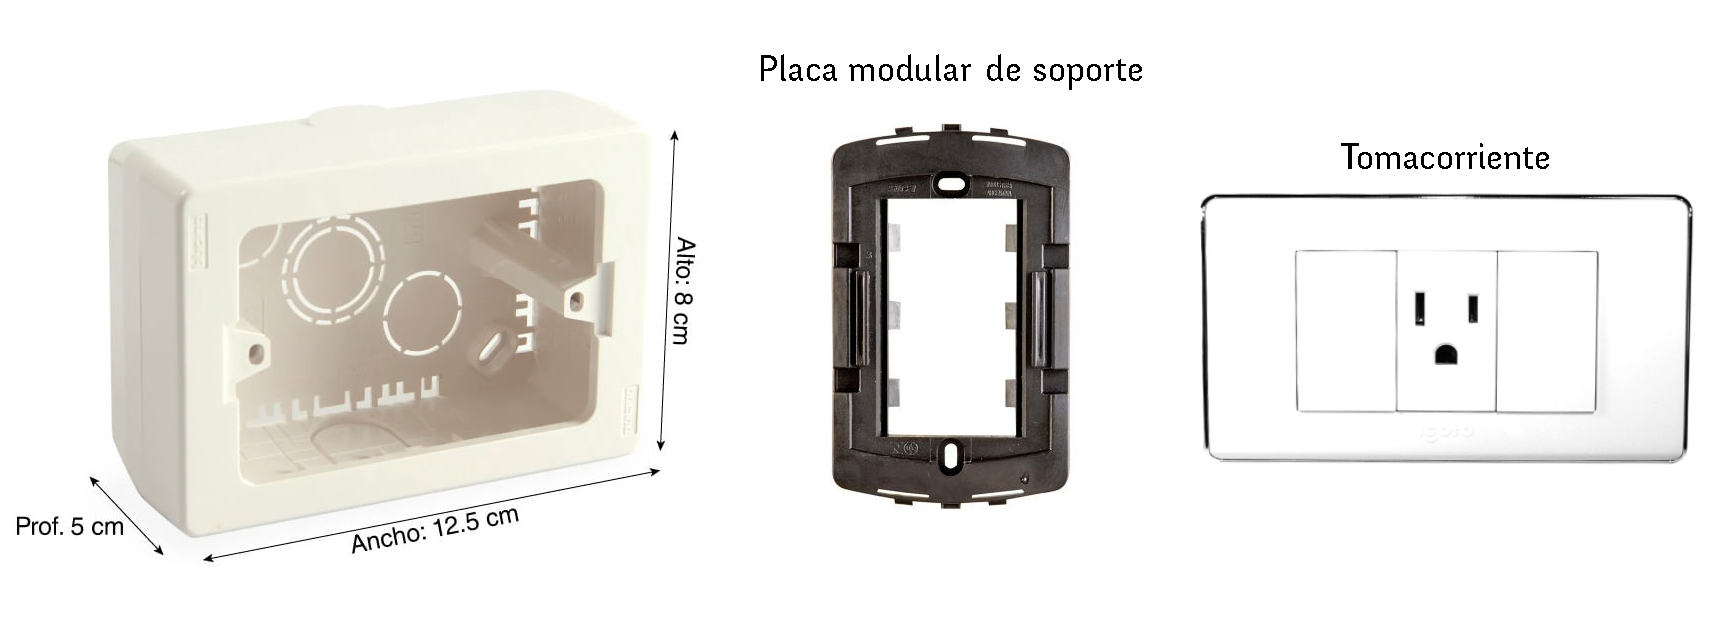
\includegraphics[width=1.0\textwidth]{./Figures/actuador.jpg}
\caption{Case del módulo actuador.}
\label{fig:caseactuador}
\end{figure}


\begin{figure}[htpb]
\centering 
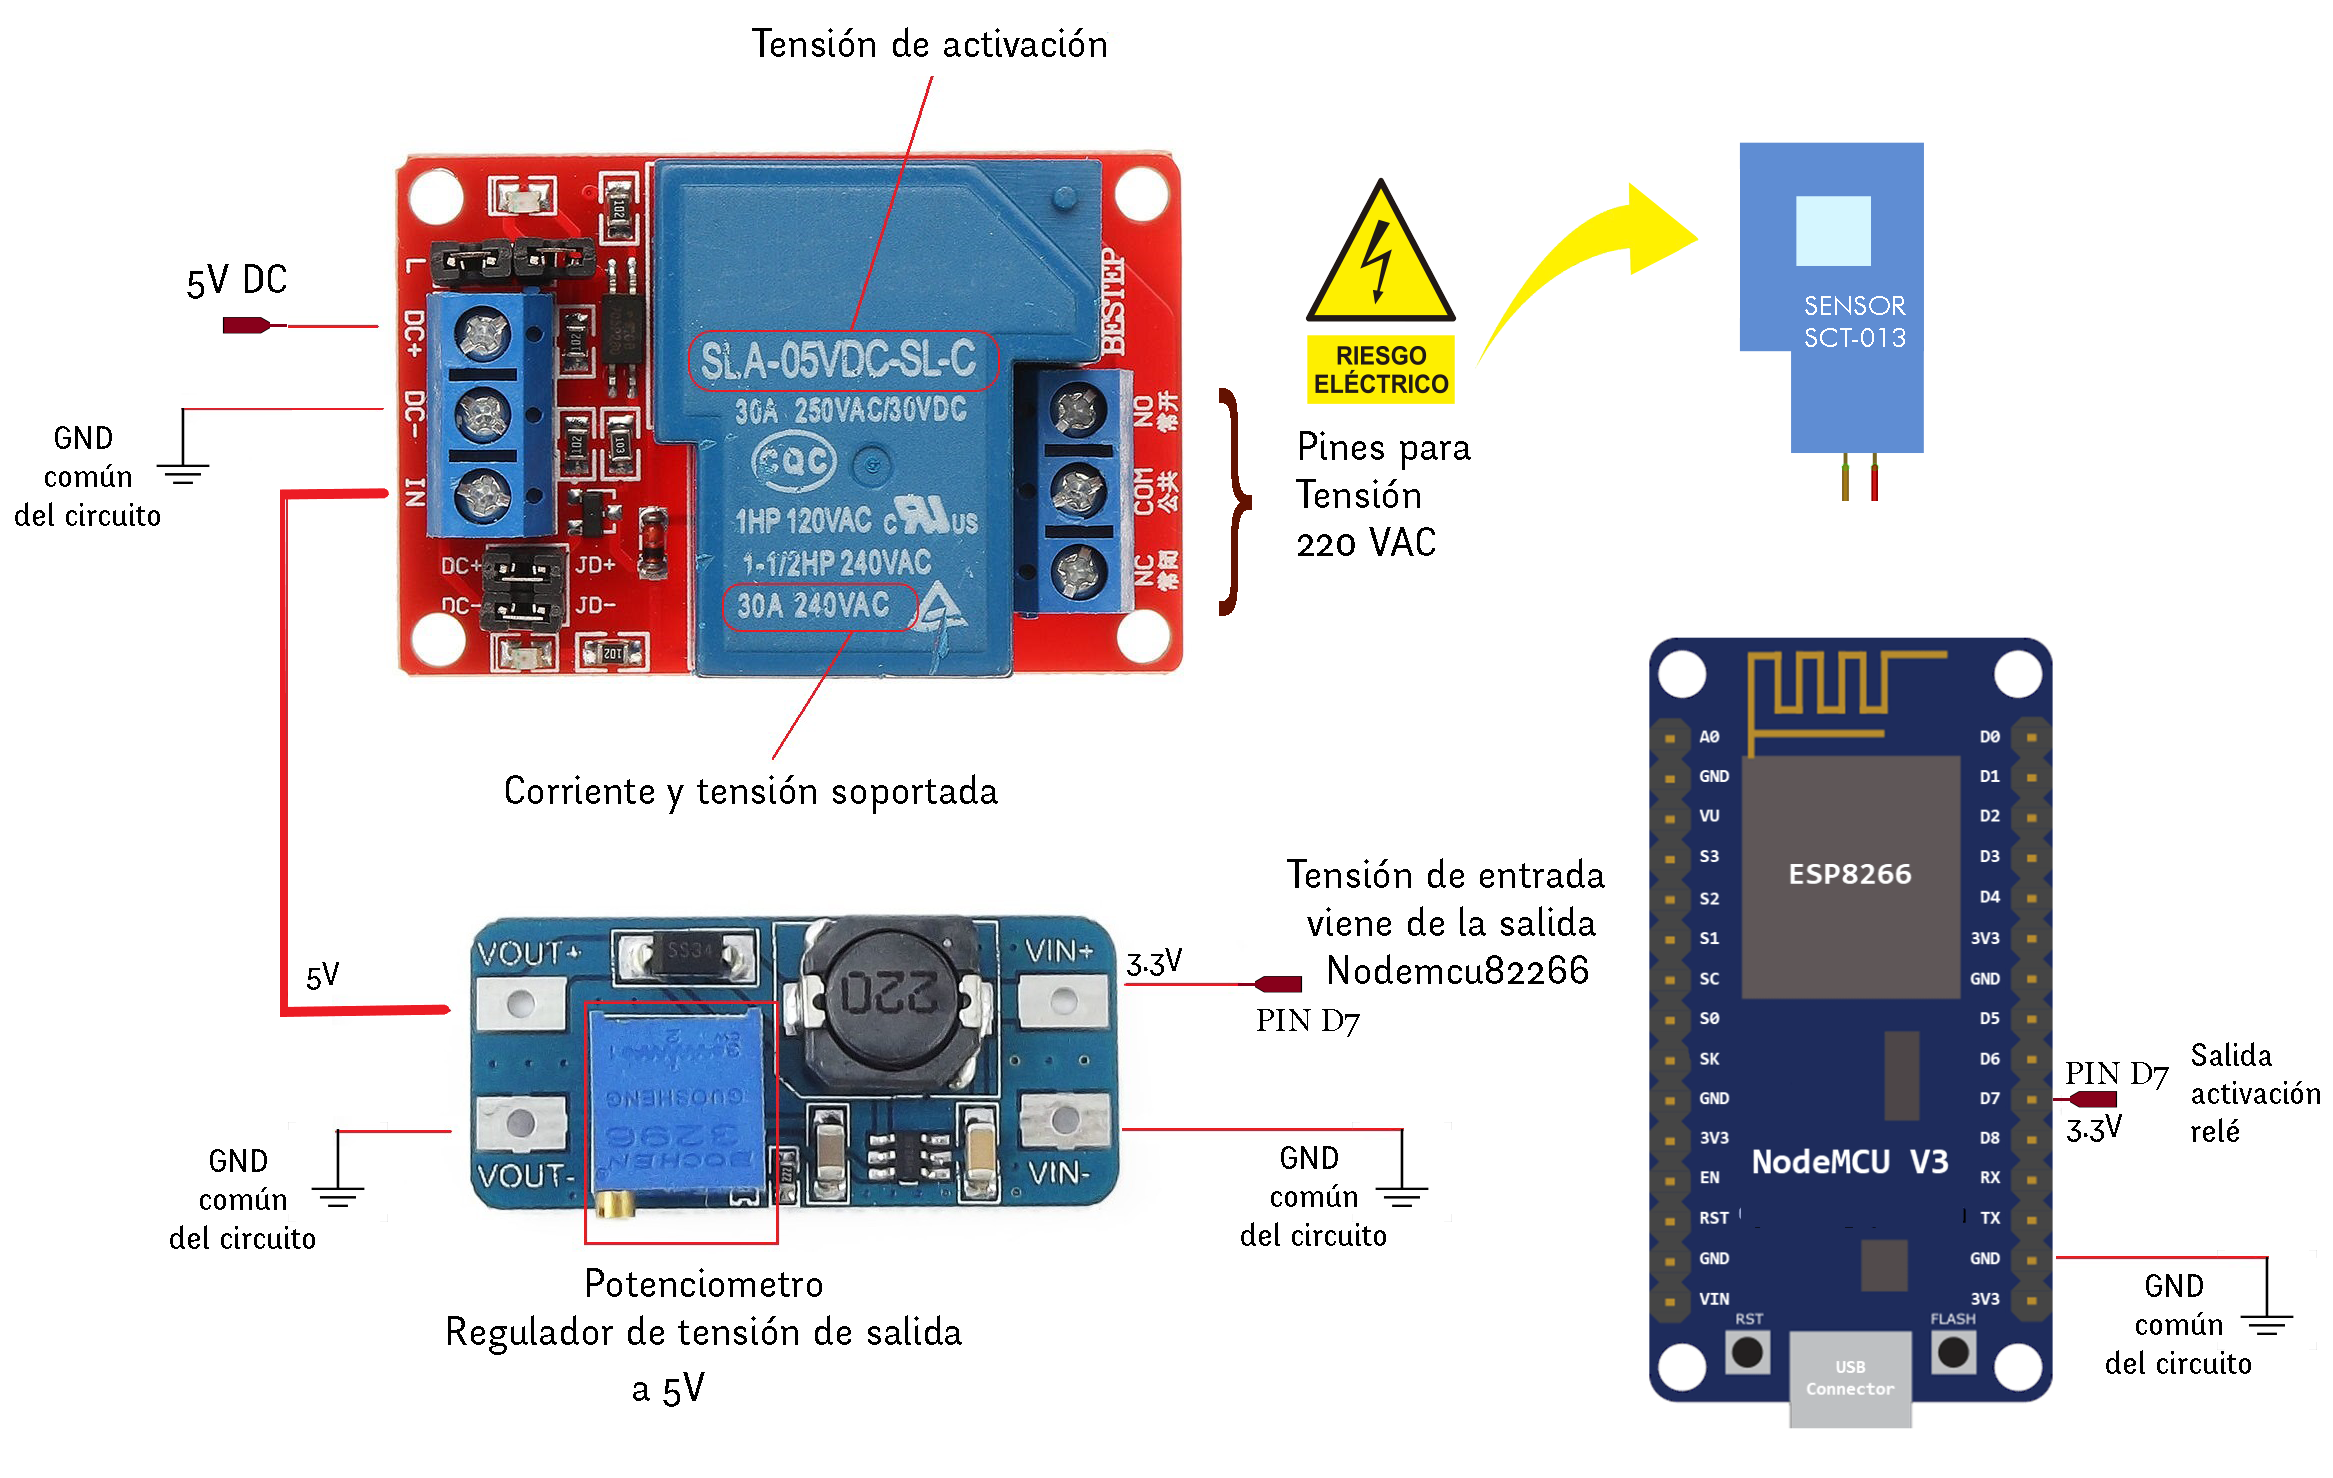
\includegraphics[width=1.0\textwidth]{./Figures/esquemaactuador.png}
\caption{Uso del Step-Up DC-DC para activación del relé. }
\label{fig:esquemaactuador}
\end{figure}

%\vspace{1cm}
%\vspace{1cm}

\section{Módulo de consumo eléctrico}

Este módulo es el responsable de medir el consumo de energía eléctrica dentro de un hogar, oficina o edificio. Este módulo fue desarrollado para permitir la comunicación bidireccional entre el módulo y el servidor local por la necesidad de sincronización con todos los clientes actuadores conectados al sistema.

%\vspace{2cm}

\keyword{Cálculo de consumo de energía eléctrica}

La energía que consume un artefacto eléctrico, se determina multiplicando la potencia de dicho artefacto por la cantidad de horas que está encendido \citep{BOOK:3}. Por ejemplo ver la ecuación \ref{eq:consumoform}.

\begin{equation}
	\label{eq:consumoform}
	EC = \left( P \cdot T \right)
\end{equation}

\vspace{0.1cm}
Siendo las variables y unidades:
\begin{itemize}
\item EC: energía consumida (kWh)
\item T: tiempo que esta encendido (h)
\item P: potencia eléctrica del artefacto (kW)
\end{itemize}

\vspace{0.1cm}
\keyword{Cálculo de la potencia eléctrica}

El cálculo de la potencia eléctrica se obtiene multiplicando la carga eléctrica, también conocida como tensión eléctrica, que pasa en un instante de tiempo a través de una diferencia de potencia, denominada intensidad. El resultado, cuya unidad es el vatio (en inglés, watt) su símbolo es la W, se obtiene al multiplicar la tensión por la intensidad. La tensión se pone en Voltios (V) y la intensidad en Amperios (A). La fórmula de la potencia eléctrica se ilustra en la ecuación \ref{eq:potenciaform} \citep{WEBSITE:20}.

\begin{equation}
	\label{eq:potenciaform}
	P = \left( V \cdot I \right)
\end{equation}

\vspace{0.2cm}
Siendo las variables y unidades:
\begin{itemize}
\item V: tension eléctrica (V)
\item I: intensidad eléctrica (A)
\item P: potencia eléctrica del artefacto (W)
\end{itemize}


Como se observa en la ecuación \ref{eq:potenciaform}, para poder medir el consumo eléctrico se necesita medir la tensión (V) y la intensidad (A), para lo que se utilizaron los sensores SCT-013-030 y  AC - ZMPT101B, respectivamente.

Los aspectos más importantes para el diseño, desarrollo y construcción del módulo de consumo eléctrico se describen  a continuación:


\begin{enumerate}
\item \keyword{Componentes para la construcción del módulo}

Los elementos necesarios fueron:
\begin{itemize}
\item Gabinete de protección.
\item Sensor de tensión eléctrica AC - ZMPT101B.
\item Sensor de corriente eléctrica SCT-013-030.
\item Convertidor ADC ADS1115.
\item Cable de calibre 14.
\item Fusible de 30 A.
\item Pantalla gráfica LCD.
\item Fuente embebida con entrada 220 V y salida de 5 V.
\item Leds ultra brillantes.
\end{itemize}

\item \keyword{Aplicación del sensor SCT-013-030}

Para este trabajo se utilizó el sensor de salida por tensión SCT-013-030 que soporta corrientes máximas de 30 A (30 A /1 V) y salida en tensión de 1 V.A. Una intensidad de 30 A a 230 V corresponde con una carga de 6.900 W, potencia suficiente para la mayoría de usuarios domésticos. En la figura \ref{fig:consumo1} se ilustra el esquema lógico a usar y la pinza del sensor.
\vspace{0.5cm}
\begin{figure}[htpb]
\centering 
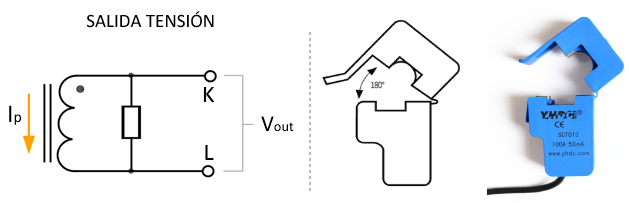
\includegraphics[width=0.9\textwidth]{./Figures/consumo1.png}
\caption{Circuito y pinza del sensor de corriente. }
\label{fig:consumo1}
\end{figure}

El proceso de ensamblado se ilustra en las fotografías de la figura \ref{fig:armadoactuador}.

\begin{figure}[htpb]
\centering 
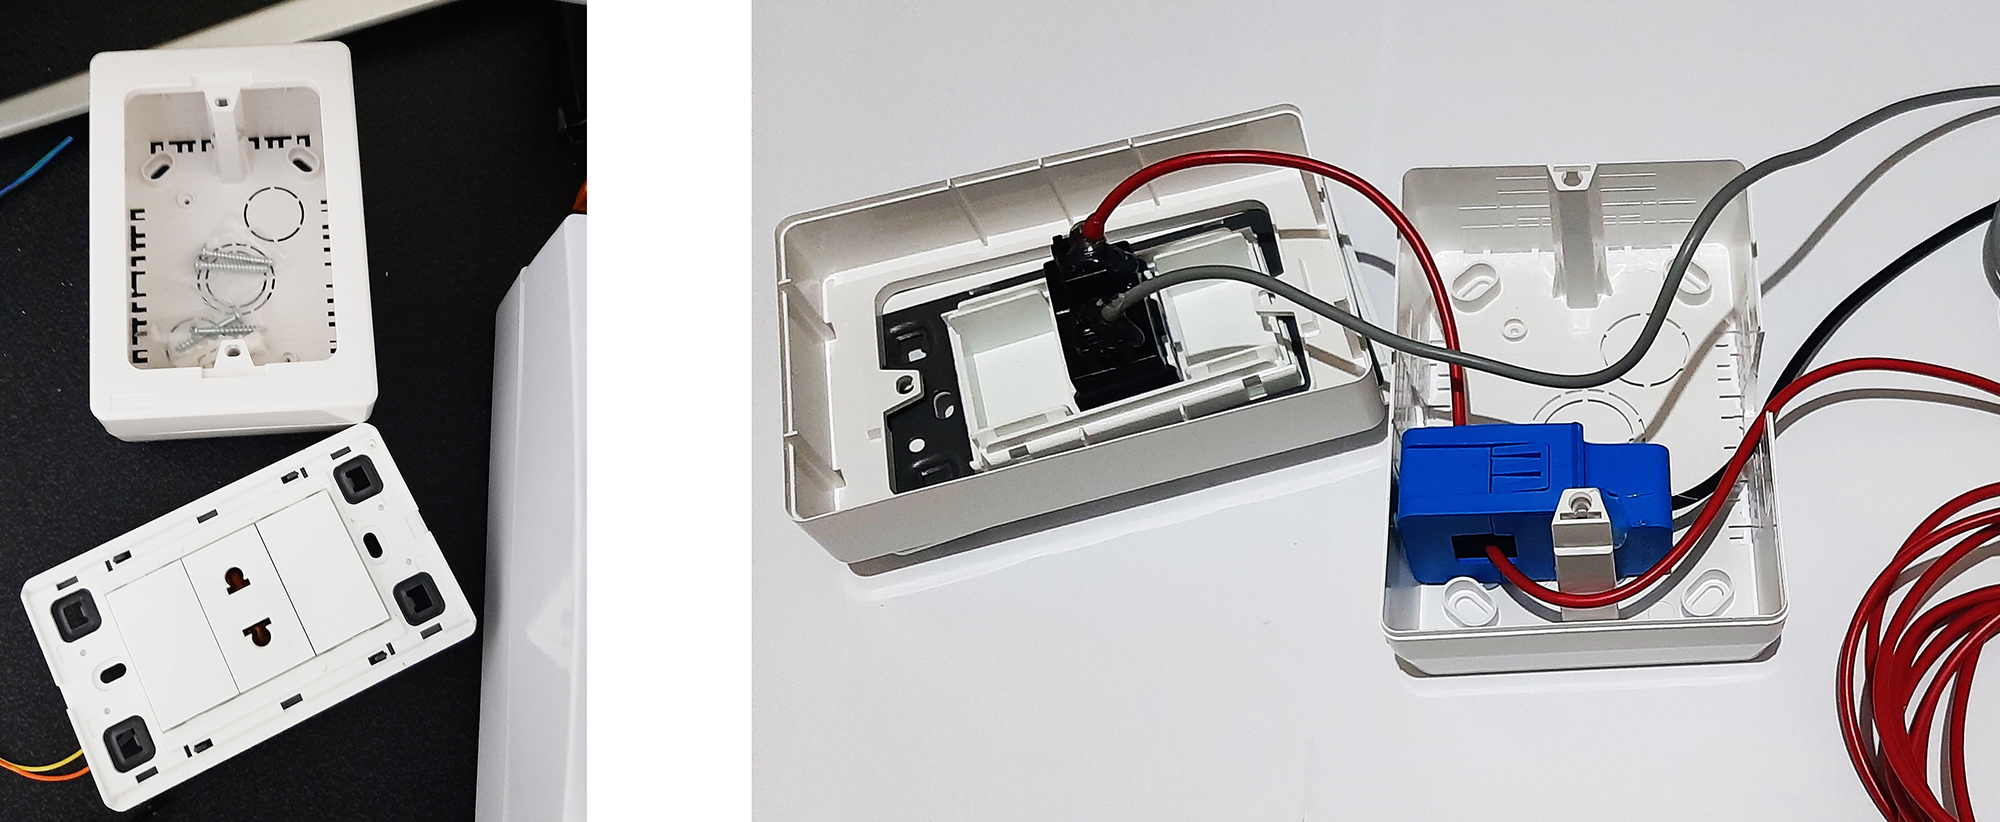
\includegraphics[width=0.85\textwidth]{./Figures/armadoactuador.jpg}
\caption{Ensamblado del módulo actuador. }
\label{fig:armadoactuador}
\end{figure}


\item \keyword{Medición del consumo eléctrico}

Para determinar la potencia eléctrica consumida, el sistema recolecta mediciones del sensor de consumo y realiza la operación matemática de la formula \ref{eq:potenciaform}. Los resultados los almacena de forma periódica (aproximadamente cada 2 segundos) en la base de datos local y remota. Los datos son agrupados según la hora de lectura junto a su respectiva fecha. La tabla \ref{tab:tablaconsumos} muestra la lógica de registros.




\begin{table}[h]
	\centering
	\caption[Registros de consumos]{Registros de consumos}
	\begin{tabular}{l c c }     
		\toprule
		\textbf{Potencia electrodoméstico} & \textbf{Respaldo} &\textbf{Fecha} \\
		\midrule
		Potencia media del ventilador (Pmv) & 10:00 am & 01/02/2022\\		
		Potencia media del ventilador (Pmv) & 11:00 am &01/02/2022 \\
		Potencia media del ventilador (Pmv) & 2:00 pm & 01/02/2022\\		
		Potencia media del ventilador (Pmv) & 3:00 pm & 01/02/2022\\		
		
		\bottomrule
		\hline
	\end{tabular}
	\label{tab:tablaconsumos}
\end{table}

Cada agrupación tiene un aproximado de 1800 registros temporales obtenidos en una determinada hora. Si se considera como ejemplo los datos de la tabla \ref{tab:tablaconsumos}, el consumo del ventilador en el día 01/02/2022 se calcula usando la formula \ref{eq:consumoform}, dando como resultado la ecuación \ref{eq:potenciaformejemplo2}.

\begin{equation}
	\label{eq:potenciaformejemplo2}
	EC =  \left( P \cdot T \right) = \left(Pmv \cdot 4 \right)
\end{equation}

Los valores del consumo total serán usados para generar la facturación mensual por consumo eléctrico. La figura \ref{fig:modconsumo} muestra la construcción del módulo de consumo.

\begin{figure}[htpb]
\centering 
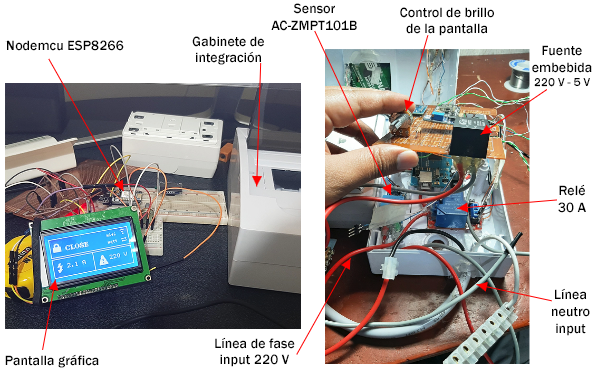
\includegraphics[width=1.0\textwidth]{./Figures/moduloconsumo.png}
\caption{Construcción del módulo de consumo.}
\label{fig:modconsumo}
\end{figure}


\end{enumerate}
\section{Módulo réplica}
Este módulo es una copia del software de monitoreo y control local y esta ubicado en la nube. Utiliza los servicios de un servidor y un broker remoto.

%\vspace{1.0cm}



%%%%%%%%%%%%%%%%%%%%%%%%%%%%%%%%%%%%%%%%%%%%%%%%%%%%%%%%%%%%%%%%%%%%%%%%%%%%%
%\begin{landscape} % esto es para rotar la pagina e imagen
%\begin{figure}[htpb]
%\centering 
%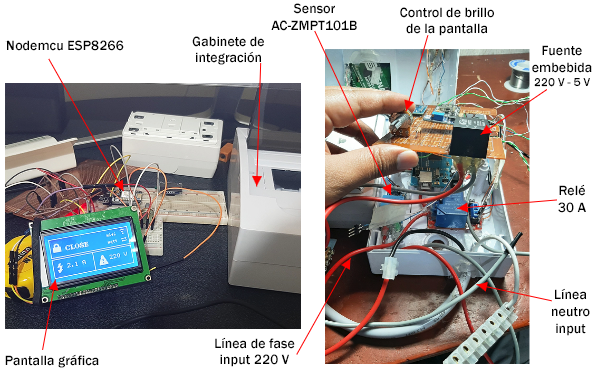
\includegraphics[width=1.5\textwidth]{./Figures/moduloconsumo.png}
%\caption{Construcción del módulo de consumo.}
%\label{fig:modconsumo}
%\end{figure}
%\end{landscape} % 
%%%%%%%%%%%%%%%%%%%%%%%%%%%%%%%%%%%%%%%%%%%%%%%%%%%%%%%%%%%%%%%%%%%%%%%%%%%%%%
\section{Diseño de la red IoT}

Para el diseño de la red se agregó un router inalámbrico como punto de acceso adicional a la red local, sirviendo como medio de comunicación exclusivo de los sensores y actuadores del sistema dentro de la red interna del hogar o edificio. La figura \ref{fig:diagramared} ilustra el diseño físico de la red utilizada.
%\vspace{0.5cm}
%%%%%%%%%%%%%%%%%%%%%%%%%%%%%%%%%%%%%%%%%%%%%%%%%%%%%%%%%%%%%%%%%%%%%%%%%%%%%
%\begin{landscape} % esto es para rotar la pagina e imagen
\begin{figure}[htpb]
\centering 
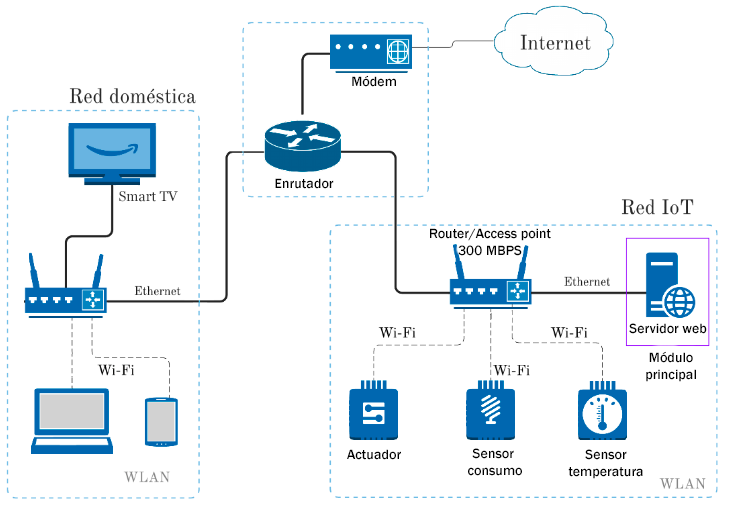
\includegraphics[width=1.0\textwidth]{./Figures/rediot3.png}
\caption{Diseño físico de la red IoT para el sistema.}
\label{fig:diagramared}
\end{figure}
%\end{landscape} % 
%%%%%%%%%%%%%%%%%%%%%%%%%%%%%%%%%%%%%%%%%%%%%%%%%%%%%%%%%%%%%%%%%%%%%%%%%%%%%
% se retira la seccion de configuración wlan
%%%%%%%%%%%%%%%%%%%%%%%%%%%%%%%%%%%%%%%%%%%%%%%%%%%%%%%%%%%%%%%%%%%%%%%%%%%%%
\section{Diseño del software para monitoreo y control}

El software desarrollado para este trabajo fue diseñado e implementado a medida por ser parte fundamental dentro de los objetivos planteados al inicio. El software es de tipo web y cumple con la característica de ser un diseño responsivo para garantizar la correcta visualización en los distintos dispositivos del mercado actual. La figura \ref{fig:patrondiseniosoftware} muestra el patrón a seguir en el desarrollo de las interfaces gráficas de usuario (GUI) del software.

\begin{figure}[htpb]
\centering 
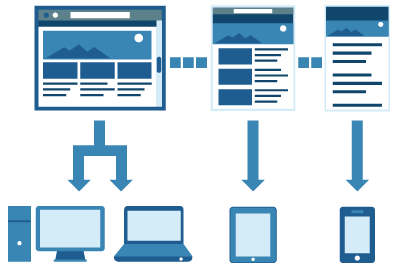
\includegraphics[width=0.75\textwidth]{./Figures/responsive3.png}
\caption{Patrón del diseño web responsivo para el \emph{software} \protect\footnotemark.}
\label{fig:patrondiseniosoftware}
\end{figure}

\footnotetext{Imagen tomada de \url{https://www.genbeta.com/desarrollo/responsive-design-introduccion}}


\section{Almacenamiento de los datos}

El sistema de monitoreo utiliza una base de datos para almacenar los valores de sensores y consumos. Por consiguiente, para este trabajo fue necesaria la creación de una base de datos para almacenar los valores que se generan por todos los módulos de sensores y actuadores. 

El gestor de base de datos elegido fue MySQL por ser de característica \emph{software} libre y ofrecer alta compatibilidad de conexión con el lenguaje \emph{backend} utilizado. El modelo entidad relación implementado en la base de datos se muestra en la figura \ref{fig:entidadrelacion}:

\begin{figure}[htpb]
\centering 
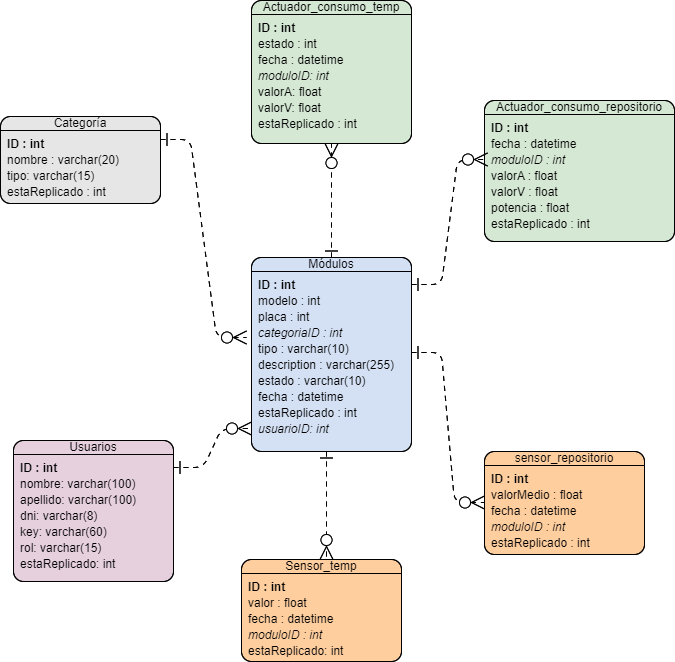
\includegraphics[width=1.0\textwidth]{./Figures/entidad-relacion.png}
\caption{Modelo entidad relación de la base de datos.}
\label{fig:entidadrelacion}
\end{figure}